\documentclass[tikz,border=2pt]{standalone}
\usepackage{amsmath,amssymb}
\usetikzlibrary{arrows.meta}
\begin{document}
% (s,S) = (2,8) policy, lead time l = 2, demands 2,3,1,4,0,3,2,5,1,2 in periods 1..10.
% Each period k shows the start value (left half) and the end value after the demand (right half).
% Inventory position P (dashed) jumps when an order is placed; inventory level I (solid) jumps l = 2
% periods later when it arrives; the gap P_k - I_k is the quantity on order.
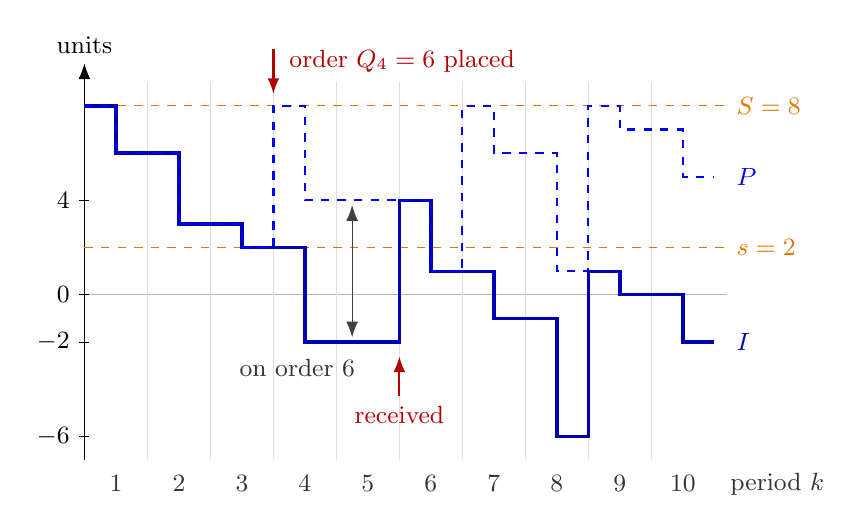
\begin{tikzpicture}[font=\small, >={Latex[length=2mm]}, x=0.8cm, y=0.3cm]
  % axes
  \draw[gray!60] (0,0) -- (10.2,0);
  \draw[->] (0,-7) -- (0,9.8) node[above] {units};
  \foreach \v in {-6,-2,0,4} {\draw (0.08,\v) -- (-0.08,\v) node[left] {$\v$};}
  \foreach \k in {1,...,10} {\node[gray!40!black] at (\k-0.5,-8) {$\k$};}
  \node[gray!40!black, anchor=west] at (10.1,-8) {period $k$};
  \foreach \k in {1,...,9} {\draw[gray!25] (\k,-7) -- (\k,9);}
  % policy levels
  \draw[orange!90!black, thin, dashed] (0,8) -- (10.2,8) node[right] {$S=8$};
  \draw[orange!90!black, thin, dashed] (0,2) -- (10.2,2) node[right] {$s=2$};
  % inventory level I (solid) and inventory position P (dashed)
  \draw[blue!70!black, very thick] (0,8) -- (0.5,8) -- (0.5,6) -- (1,6) -- (1.5,6) -- (1.5,3) -- (2,3) -- (2.5,3) -- (2.5,2) -- (3,2) -- (3.5,2) -- (3.5,-2) -- (4,-2) -- (4.5,-2) -- (5,-2) -- (5,4) -- (5.5,4) -- (5.5,1) -- (6,1) -- (6.5,1) -- (6.5,-1) -- (7,-1) -- (7.5,-1) -- (7.5,-6) -- (8,-6) -- (8,1) -- (8.5,1) -- (8.5,0) -- (9,0) -- (9.5,0) -- (9.5,-2) -- (10,-2);
  \draw[blue, thick, dashed] (0,8) -- (0.5,8) -- (0.5,6) -- (1,6) -- (1.5,6) -- (1.5,3) -- (2,3) -- (2.5,3) -- (2.5,2) -- (3,2) -- (3,8) -- (3.5,8) -- (3.5,4) -- (4,4) -- (4.5,4) -- (5,4) -- (5.5,4) -- (5.5,1) -- (6,1) -- (6,8) -- (6.5,8) -- (6.5,6) -- (7,6) -- (7.5,6) -- (7.5,1) -- (8,1) -- (8,8) -- (8.5,8) -- (8.5,7) -- (9,7) -- (9.5,7) -- (9.5,5) -- (10,5);
  % labels of the two paths
  \node[blue, anchor=west] at (10.2,5) {$P$};
  \node[blue!70!black, anchor=west] at (10.2,-2) {$I$};
  % order placed at the start of period 4 and received at the start of period 6
  \draw[red!70!black, ->, thick] (3,10.4) -- (3,8.5);
  \node[red!70!black, anchor=west] at (3.1,9.9) {order $Q_4=6$ placed};
  \draw[red!70!black, ->, thick] (5,-4.3) -- (5,-2.6);
  \node[red!70!black, anchor=north] at (5,-4.3) {received};
  % gap = quantity on order in period 5
  \draw[gray!50!black, <->] (4.25,-1.8) -- (4.25,3.8);
  \node[gray!40!black, anchor=north east] at (4.45,-2.3) {on order $6$};
\end{tikzpicture}
\end{document}
